\documentclass[a4paper, 11pt]{article}
\usepackage{geometry}
\usepackage{indentfirst}
\usepackage{setspace}
\usepackage{amsmath}
\usepackage{graphicx}
\usepackage{wrapfig}
\usepackage{caption}
\usepackage{indentfirst}
\setlength{\parindent}{20pt}
\usepackage{amssymb}
\usepackage{float}
\usepackage{subcaption}

\graphicspath{ {./images/} }
\geometry{left=2.5cm, right=2.5cm, top=2.5cm, bottom=2.5cm}

\begin{document}	
	\title{Exercise \# 3. Numerical Solution of the Poisson Problem. }
	\author{{\small Alexandre Rodrigues (2039952)}}
	\date{\today}
	
	\maketitle
		\section{Method}
			I will describe relevant steps of developing this implementation and respective theory.
			Based on the homework text I implemented each step in Matlab.
			
			\begin{enumerate}
				\item \textbf{Input files from specified mesh:}
					\subitem \textbf{1.} The user selects a mesh refinement level (0 to 4);
					\subitem \textbf{2.} All 3 files are loaded: \texttt{topol}, \texttt{bound} and \texttt{coord}.	
				
				\item \textbf{create pattern for the stiffness matrix:} 
					\subitem \textbf{1.} I created a range vector 1 to \texttt{Ne}, then place it 3 times as a column in a matrix and reshaped the matrix to obtain the column vector $ row = [1,1,1,2,2,2,3,\ldots]^T $. 
					\subitem \textbf{2.} The \texttt{col} vector is simply obtained by reshaping the \texttt{topol} as a column vector. 
					\subitem \textbf{3.} Then we can compute the adjacency matrix as \texttt{A = sparse(row,col,1)} and the pattern for the stiffness matrix as \texttt{H = A' * A}, finally we clean the matrix as we only want the sparse pattern, \texttt{H = H * 0}.
				
				\item \textbf{Stiffness matrix:}
					I created the function \texttt{[H, delta] = computeStiff(H, topol, coord)} to encapsulate all the following computations.
					It has the topology and coordinates matrices as inputs, as well as the $ H $ matrix with its pattern already defined before.
					Its outputs are the final $ H $ matrix and the \texttt{delta} vector with the surface measures of each element.
					Using a for loop for each element:
					\subitem \textbf{1.} Get coordinates of the 3 nodes that define the element, compute the surface measure for that element and save it in the \texttt{delta} vector.
					$$ \Delta = \frac{1}{2} \begin{vmatrix} 1 & x_i & y_i \\ 1 & x_j & y_j \\ 1 & x_m & y_m \end{vmatrix} $$
					\subitem \textbf{2.} Compute the $ b $ and $ c  $ coefficients of the basis functions ($a$ is not needed): 
					$$  b_i = y_j - y_m  \qquad c_i = x_m - x_j ,$$ others are obtained using anticlockwise indices permutation.
					\subitem \textbf{3.} Compute \texttt{Hloc} for an element as 
					$$ H_{loc} = \frac{1}{4\Delta}\{ b^Tb + c^Tc \} $$ 
					where $ b = [b_i, b_j, b_m]$ and $ c = [c_i, c_j, c_m]$
					\subitem \textbf{4.} Assemble the stiffness matrix H from the local matrices using algorithm 3.3.
				
				\item  \textbf{Right hand size:}
					Using a for loop to iterate in the list of nodes:
					\subitem \textbf{1.} Get the node coordinates;
					\subitem \textbf{2.} Find elements that have this node as a vertex and get their surface measures from the \texttt{delta} vector;
					\subitem \textbf{3.} Compute the right hand size vector as $f_i \approxeq (-4 +2x_i^2 + 2y_i^2)  \frac{\sum_e \Delta_e}{3} $
				
				\item \textbf{Boundary Conditions:}
					As explained in the homework text we can simply change the diagonal value \texttt{H(i,i)}.
					So I changed the diagonal value of $ H $ at the node \texttt{i} of the boundary, \texttt{H(i,i)=Rmax}.
				
				\item \textbf{Solve the Linear System:}
					Following recommendations I used tolerance as $ 1 \times 10^{-8} $ and Matlab's PCG method, Jacobi preconditioner as \texttt{M = sparse(diag(diag(H)))}, Choledsky preconditioner as \texttt{L = ichol(H)}.
					Then we can call the PCG method to solve the linear system.
				
				\item \textbf{Error computation:} Using a for loop to visit each node:
					\subitem \textbf{1.} Get the coordinates of the node;
					\subitem \textbf{2.} Compute the analytical solution as $u(x,y) = x^2 + y^2 - x^2y^2 - 1$;
					\subitem \textbf{3.} Sum surface measures of each element that have this node as a vertex;
					\subitem \textbf{4.} Compute local error as $ (u_i - u(x_i,y_i)^ 2 \frac{\sum_e \Delta_e}{3} $;
					\subitem \textbf{5.} Sum all the local errors and $ \epsilon $ will be its square root.	
			\end{enumerate}
			
	
		
		\section{Results}
		
			\subsection{Convergence Plots}
			
				As required the following images show the convergence plots for all refinement levels, one for each preconditioner.
				
				\begin{figure}[H]
					\begin{subfigure}{.49\textwidth}
						\centering
						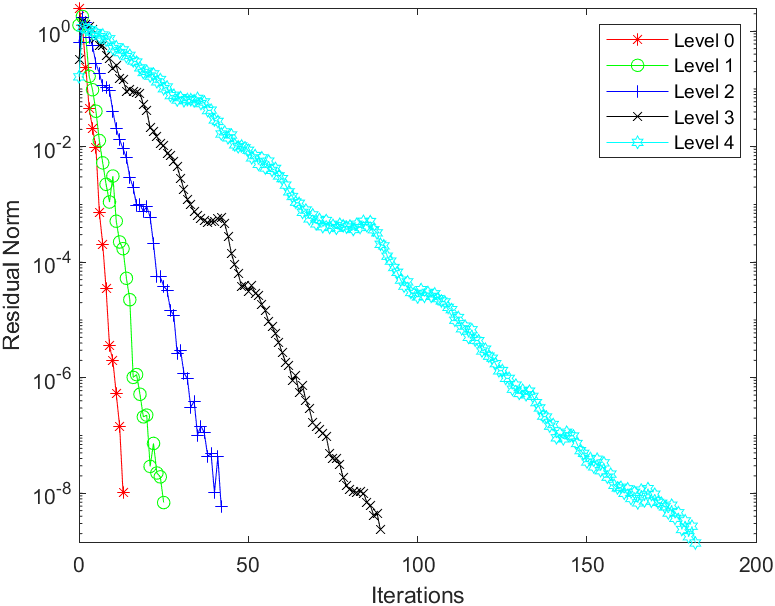
\includegraphics[width=.99\linewidth]{ConvergenceJ.png}  
						\caption{Jacobi}
						\label{fig:Jacobi}
					\end{subfigure}
					\begin{subfigure}{.49\textwidth}
						\centering
						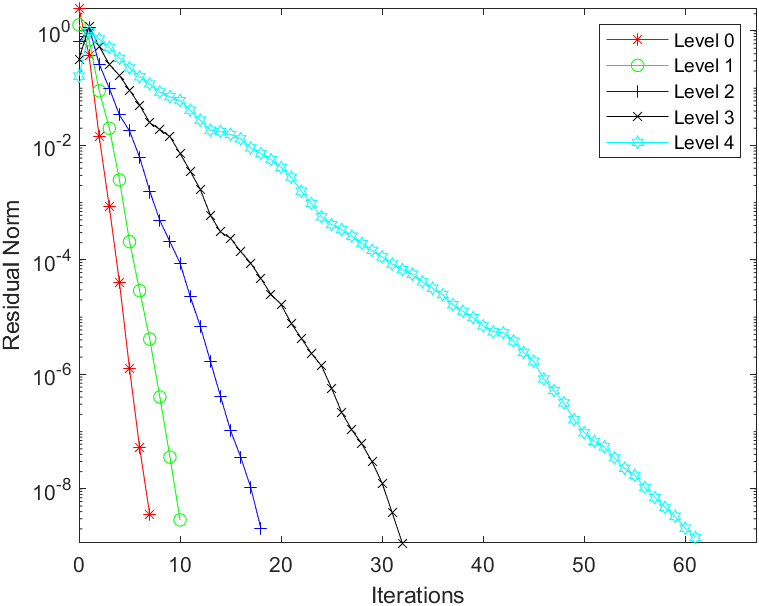
\includegraphics[width=.99\linewidth]{ConvergenceC.png}  
						\caption{Choledsky}
						\label{fig:Chol}
					\end{subfigure}
					\caption{Convergence plots - Residual norms vs Iterations}
					\label{fig:convergence}
				\end{figure}
				
				There are clear differences in convergence regarding the preconditioner used.
				The Choledsky preconditioner significantly improves convergence by reducing the number of iterations needed in up to 3x.
				
				There is also a clear slowdown of convergence when increasing the level of refinement.
			
				I also recorded the computational time needed to solve each PCG method but found no relevant differences.
				
			\subsection{Error}
				\begin{table}[H]
					\centering
					\begin{tabular}{c|c|c}         
						\textbf{Level} 	& \textbf{ Error $ \epsilon $} 		& \textbf{Error Ratio}  \\ \hline
						$ 0  $			& $ 6.912 \times 10^{-2} $ 	& N/A \\ \hline
						$ 1  $			& $ 1.631 \times 10^{-2} $ 	& $ 0.236 $ \\ \hline
						$ 2  $			& $ 3.984 \times 10^{-3} $ 	& $ 0.244 $ \\ \hline
						$ 3  $			& $ 9.883 \times 10^{-4} $	& $ 0.248 $ \\ \hline
						$ 4  $			& $ 2.465 \times 10^{-4} $ 	& $ 0.249 $ \\ 
					\end{tabular}
					\caption{FEM Convergence table}
					\label{table:errors}
				\end{table}
				Each level of refinement decreases $ l $ by a factor of $ 2 $, $ l_{i+1} = \frac{1}{2}l_i $.
				The error is proportional to $l^2$ so $ \epsilon_{i+1} = \frac{1}{4}\epsilon_i $.
				This corresponds to our experimental values and ratio.
	
	
\end{document}



